
\section{Background}
\label{sec:background}

Stochastic gradient descent is a common algorithm in the field of machine
learning and thus, there are multiple off-the-self regression solvers which
utilize this approach available for use. Examples include software 
such as Matlab or, as used in this experiment, the scikit-learn library for Python.\\

The scikit-learn library provides variations of gradient descent along with 
a range of other methods such as ordinary least squares and logistic regression. 
The particular regression solver used in this experiment is a RandomizedSearchCV 
with a Ridge estimator object. In other words, we invoke a randomized search of 
hyper parameters, "free variables", while using a cross-validation scheme under 
the constraints of ridge regression. Details of these particular features will be
further discussed in the background.\\

One thing that our model shares with the other machine learning models  is
the use of a cost-function. Cost-functions vary from model to model, but they all 
penalize errors made in predictions. The predictions are made with a hypothesis 
function, $h(\theta)$, specific to the data under investigation. The value of any 
prediction can then be used in a cost function to determine the quality of the model. 
Only penalizing for error, the cost function is represented as: 
$$J(\vec{\theta}) = \frac{1}{2m} [\sum_{i = 1}^{m} (y^{(i)} - h(\theta))^2]$$
However, as representations add higher-order terms, 
the cost function may be augmented to penalize for complexity as well.


\subsection{Regularization}

Our initial model uses $L_{2}$ Regularization, otherwise known as ridge regression.
Regularization inhibits models from becoming too complex. The complexity of an equation is determined by the order of the polynomials present and the size of coefficients; smaller coefficients reduce the impact of higher order polynomials on the curve and thus reduce drastic changes in the value $x_{2}$ based on changes in $x_{1}$.\\

The added concern for complexity calls for a change in the cost function. Under the
experiments carried out in this project, the cost function becomes: 
$$J(\vec{\theta}) = \frac{1}{2m} [\sum_{i = 1}^{m} (y^{(i)} - h(x^{(i)})^2 + \alpha \| \theta ^ 2 \|]$$

where $\alpha$ represents the regard for complexity. A higher $\alpha$ value
reduces complexity by driving down the weights attributed to higher older polynomial
values \cite{scikit}. \\ 

Why worry about complexity? The higher order a polynomial, the worse the 
function generalizes to new data points. A higher order polynomial may fit
exceptionally well with test data, but poorly predict new values. This is called
overfitting. On the other hand, there is a risk of underfitting data. When the model
underfits data, the model poorly predicts values in all of the training, validation, and test sets.
An example of overfitting and underfitting data sets can be seen in Fig \ref{fig:fitting}. A good fit is usually determined to have both low complexity and low error. 

\begin{figure}[htb]

  \centering  % centers the image in the column

  % replace the second argument below with your filename. I like to
  % place all my figures in a sub-directory to keep things organized
  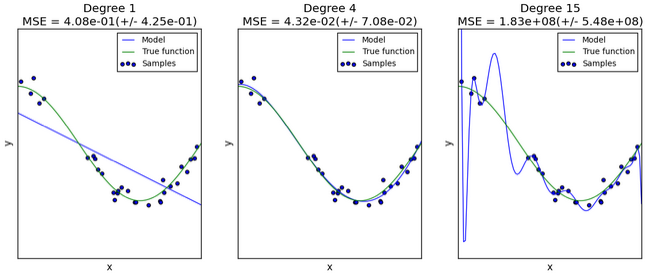
\includegraphics[width=0.47\textwidth]{figs/fitting.png}

  % *Every* figure should have a descriptive caption.
  \caption{L: Underfitting, M: Neither underfitting nor overfitting,
  		R: Overfitting. Image courtesy of \texttt{scikit-learn}.}

  % The label is a handle you create so that you can refer to this
  % figure (using the \ref{} command) from other parts of your
  % document. LaTeX automatically renumbers figures and updates
  % references when you recompile, so you should do it this way rather
  % than hard-coding in references. Notice that I've also been
  % creating labels for the various sections in the document; I could
  % use \ref{} command to refer to those sections using their labels
  % too.
  \label{fig:fitting}

\end{figure}

\subsection{A Variant}
Another type of Regularization is known as $L_{1}$ Regularization. While $L_{2}$
Regularization squares the value of the $\theta$ value, $L_{1}$ takes the absolute 
value of $\theta$ and multiplies it by $\alpha$. This is expressed by the following equation:
$$J(\vec{\theta}) = \frac{1}{2m} [\sum_{i = 1}^{m} (y^{(i)} - h(x^{(i)})^2 + \alpha \| \theta \|]$$
However, gradient descent cannot be 
used with $L_{1}$ since all parameters would shrink to a small size. This type of 
regression is known as Lasso Regression. Another feature of Lasso Regression, is that it is a sparse model. In other words, some of the final weights given to certain attributes in the final model used to predict new values. Some of the values shrink to 0, meaning only some of the features used to predict the final $x_{2}$ value will be utilized.
In our investigation, we compare $R^{2}$
scores from our primary results using the RandomizedSearchCV method and 
ridge regression model to those produced by a lasso regression model, Lasso.
 \cite{scikit}

\subsection{Cross-Validation}

Cross-validation splits a set of data into a number of distinct and separate groups, termed k-fold. 
Each of these groups is then cycled through to represent the validation set and test sets. 
The validation error across these different groupings of data is then averaged together
to create the final validation error. Overall, cross-validation acts to better generalize the decision
function since it is tested on more than one specific data set. The model is exposed to different 
combinations of data points and is thus less likely to overfit to one group of test data. 


\subsection{Grid-Search versus Randomized-Search}
We will now discuss the process
with which hyper parameters for the equation are chosen. Two common approaches
are grid-search and randomized search. Grid-search is the most commonly used to
optimize parameters \cite{scikit}. Parameters are chosen by systematically exploring
a range of possible combinations of all parameters. This ensures that a wide
range of combinations of parameters are tested. Meanwhile, random search,
the search type investigated in this project, randomly (as the name suggests)
chooses the  set of parameters. Using at least 60 random sets of hyper parameters 
(we use 100 in our experiments) we can with $95\%$ confidence get reasonably close to the optimal
hyper parameters.\\

 Further discussions of all types of models offered by the scikit-learn can
 be read in further detail at \cite{scikit}.
